\documentclass[aps,pre,twocolumn,superscriptaddress,floatfix,longbibliography]{revtex4-2}

\usepackage{amsmath,amssymb}
\usepackage{graphicx}
\usepackage{booktabs}
\usepackage[colorlinks=true,linkcolor=blue,citecolor=blue,urlcolor=blue]{hyperref}

\graphicspath{{coupled/}}

\begin{document}

\title{Adaptive agents in a coupled queueing model:\\
phase separation, theory of mind, and the loss of universality}

\author{A. Vazquez}
\affiliation{%TODO: affiliation
}

\date{\today}

\begin{abstract}
Queueing models of human dynamics predict heavy-tailed interevent times, and
extending them to two agents sharing a task that requires simultaneous execution
yields a family of exponents $\alpha = 1 + 1/\max_j(L_j-1)$ set by the queue
lengths [Oliveira and Vazquez, Physica A \textbf{388}, 187 (2009)]. In those
models the priority assigned to the shared task is drawn from a fixed
distribution. Here we let the agents \emph{choose} it. Each agent assigns the
interacting task a priority equal to its value discounted by the estimated risk
that the partner will not participate, and estimates that risk from observation.
The resulting system is a stag hunt with a saddle-node bifurcation: a coupled
phase and an absorbing solitary phase, separated by a critical line
$R_c(L)$ that we obtain in closed form, valid only for $L-1 \le 1/c$. We
report five results. (i) Agents that additionally model \emph{the partner's
model of themselves} shift the critical line substantially, and a single such
agent suffices to hold a non-modelling partner in the coupled phase. (ii) When
the interaction opportunity is rare, coupling survives only if the partner model
is held across silent intervals rather than decaying; a model maintained without
input is what makes rare interaction viable. (iii) The scale-free interevent
statistics of the non-adaptive model survive adaptation only inside a narrow
window near the bifurcation, and only when agents retain a nonzero rate of
uninformed exploration, without which the solitary phase is strictly absorbing.
(iv) Inside that window the measured exponent is controlled by the fraction of
time spent coupled and not by $L$: adaptation destroys the universality classes,
and phase occupancy replaces $\alpha$ as the natural order parameter.
(v) At fixed parameters the outcome is bimodal but is not determined by early
noise; collapse into the solitary phase is irreversible without intervention,
and the partner-modelling capability that prevents collapse with certainty
reverses it in only about a third of cases unless the agent is also willing to
persist unilaterally for intervals far longer than a myopic evaluation
sanctions, in which case recovery becomes complete. Allowing the agent to choose
its own commitment length shows this policy to be optimal rather than imposed,
and fixes its price: recovery requires persisting for $0.74\,\tau_{\rm mem}$
independently of how unfavourable the current estimate is, and an agent adopts
it only if its horizon exceeds $1.5\,\tau_{\rm mem}$.
(vi) On a network, where each agent holds one interacting task per neighbour and
attention is scarce, the solitary phase percolates as the cost of an
unreciprocated offer grows, and high-degree nodes lose their relations first.
Comparing a triadic-closure network with its degree-preserving randomization at
matched coupled-edge fraction, local structure does not change \emph{which}
relations survive but does change how their failure is arranged: the coupled
phase fragments into clusters under triadic closure while remaining connected
without it. The transition is tractable analytically: attention divides as
$1/(k+a)$, which fixes a critical degree $k_c$ beyond which no coupled state
exists, and percolation follows the Molloy--Reed criterion with the second moment
truncated at $k_c$. Because the truncation acts at the top of the degree
distribution, scale-free contact structures are maximally vulnerable.
\end{abstract}

\maketitle

\section{Introduction}

Queueing theory has become a standard framework for the timing of human
activity~\cite{barabasi2005,vazquez2005,vazquez2006}. Representing an
individual's to-do list as a priority queue with highest-priority-first
execution produces power-law interevent time distributions
$P(\tau)\sim\tau^{-\alpha}$, with $\alpha=1$ and $\alpha=3/2$ identified as
universality classes and corroborated by electronic and postal correspondence
data~\cite{barabasi2005,oliveira2005,vazquez2006}.

Single-queue models describe an isolated individual. Many activities, however,
require two or more people at once, and interaction is known from the theory of
critical phenomena to be decisive for universality~\cite{stanley1971}. A minimal
two-agent extension~\cite{oliveira2009} gives each agent one \emph{interacting}
task $I$, executable only when both agents select it in the same step, and one
aggregate \emph{non-interacting} task $O$ standing for $L_j-1$ private tasks.
That model predicts a countable family of exponents
\begin{equation}
  \alpha = 1 + \frac{1}{\max_j (L_j-1)},
  \label{eq:alpha_iid}
\end{equation}
interpolating between $2$ and $1$: the more distracted agent sets the exponent.

In that treatment the priority of the interacting task is drawn independently
from a fixed density. This is the natural assumption if the shared activity is
exogenous, but it removes the feature that makes joint tasks distinctive: an
agent who is repeatedly stood up should stop offering. Here we make the
interacting-task priority a decision variable. The agents estimate each other's
participation rate from observation and set their priority accordingly. This
changes the object from a stochastic process into a coupled inference problem
and, as we show, changes its phenomenology substantially.

\section{Model}

\subsection{Substrate}

We retain the structure of Ref.~\cite{oliveira2009}. Agent $j\in\{A,B\}$ holds
one interacting task $I$ and one aggregate task $O$ representing $a_j \equiv
L_j-1$ private tasks. The private-task priority is the maximum of $a_j$
independent uniform variates,
\begin{equation}
  f_{O_j}(x) = a_j\, x^{a_j-1}, \qquad x\in[0,1],
\end{equation}
redrawn whenever $O$ is executed. Each agent selects the higher-priority task.
$I$ executes only if both agents select it.

\subsection{Priority as a decision}

Let $x_{I_j}$ be the priority agent $j$ assigns to the interacting task. Since
$O$ is drawn afresh each step, the probability that $j$ selects $I$ is
\begin{equation}
  p_j = \Pr\!\left(x_{O_j} < x_{I_j}\right) = x_{I_j}^{\,a_j}.
  \label{eq:reachprob}
\end{equation}
The agent controls a propensity, not a decision: with many private tasks, $a_j$
large, even a high $x_{I_j}$ yields a small participation probability.

Payoffs per step: both agents select $I$, each receives $R_I$; an agent selects
$I$ while its partner does not, it receives $x_{O_j}-c$, the step being wasted
and $c>0$ the cost of an unreciprocated offer; otherwise it receives $x_{O_j}$,
the realised value of its private task. The cost $c$ is what makes a model of
the partner necessary; at $c=0$ the optimal policy is $x_{I_j}=1$ regardless of
the partner.

Writing $\hat p$ for the agent's estimate of its partner's participation
probability, selecting $I$ is preferable whenever
$\hat p R_I + (1-\hat p)(x_{O_j}-c) > x_{O_j}$, giving the optimal priority
\begin{equation}
  x_{I_j}^{*} = \left[\, R_I - c\,\frac{1-\hat p}{\hat p} \,\right]_0^1 ,
  \label{eq:policy}
\end{equation}
where $[\cdot]_0^1$ denotes clipping to $[0,1]$: \emph{the value of the
interaction discounted by the risk that the partner will not participate}.
Estimates are maintained by an exponential moving average with retention
$\lambda=e^{-1/\tau_{\rm mem}}$ over the partner's observed selections.

\subsection{Levels of modelling}

We distinguish three policies by what each agent represents.

\begin{description}
\item[Level 0] No partner model: $x_I = R_I$, clipped.
\item[Level 1] Partner model: $\hat p$ tracked, Eq.~\eqref{eq:policy} applied.
\item[Level 2] Self model: the agent additionally tracks $\hat s$, its estimate
  of \emph{the partner's estimate of itself}, and evaluates a finite-horizon
  rollout of the coupled dynamics in which its own participation raises $\hat s$,
  which raises the partner's priority through Eq.~\eqref{eq:policy}, which raises
  the partner's participation. It commits to $x_I=1$ when that rollout dominates
  the myopic choice.
\end{description}

Level 2 is the minimal policy that requires an agent to represent itself as an
object in another agent's model.

\subsection{Exploration}

Each agent additionally participates with probability $\epsilon$ per step
irrespective of belief. This is not a numerical convenience. At $\epsilon=0$
the state $p=0$ is strictly absorbing: an agent that stops participating never
observes its partner participating and therefore never revises. Escape requires
both agents to explore in the same step, at rate $\epsilon^2$.

\section{Fixed points}

For a symmetric pair the participation probability obeys $p \mapsto
\mathcal{F}(p)$ with
\begin{equation}
  \mathcal{F}(p) = \Bigl(\left[\, R_I - c\,\frac{1-p}{p} \,\right]_0^1\Bigr)^{a}.
\end{equation}
Setting $\mathcal{F}(p)=p$ and requiring tangency gives the saddle-node in
closed form,
\begin{equation}
  p^{*} = (a c)^{a/(a+1)}, \qquad
  R_c = (p^{*})^{1/a} + \frac{c}{p^{*}} - c .
  \label{eq:rcrit}
\end{equation}
For $c=0.35$ this gives $R_c=0.8332$ at $p^*=0.5916$ for $L=2$, and
$R_c=0.9818$ at $p^*=0.7885$ for $L=3$.

Equation~\eqref{eq:rcrit} is meaningful only while $p^*\le 1$, that is
\begin{equation}
  a \le 1/c .
  \label{eq:validity}
\end{equation}
Above this bound the tangency lies outside the accessible range and there is no
interior bifurcation: the coupled phase is created discontinuously at the
clipping boundary $x_I=1$. At $c=0.35$ this restricts the continuous transition
to $L\le 3.86$. Figure~\ref{fig:phase} shows the return map and the critical
line.

Below $R_c$ only the solitary fixed point $p=0$ exists. Above it there are two
stable phases, coupled and solitary, separated by an unstable point whose
position rises with $a$: more private tasks enlarge the basin of solitude. The
structure is that of a stag hunt, with the solitary phase risk-dominant and
absorbing at $\epsilon=0$.

\begin{figure*}[t]
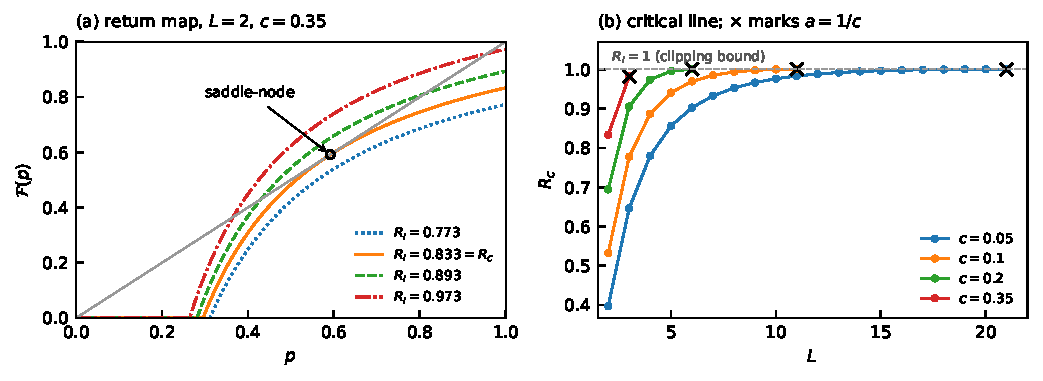
\includegraphics[width=\textwidth]{fig_phase.pdf}
\caption{(a) Return map $\mathcal{F}(p)$ for $L=2$, $c=0.35$ at several $R_I$,
with the diagonal in grey. The two nontrivial fixed points are born in a
saddle-node at $R_c=0.8332$, $p^*=0.5916$ (circle). (b) Critical line $R_c(L)$
from Eq.~\eqref{eq:rcrit} for several costs $c$; crosses mark the validity
boundary $a=1/c$, Eq.~\eqref{eq:validity}, beyond which no interior bifurcation
exists.}
\label{fig:phase}
\end{figure*}

\section{Results}

Unless stated otherwise, simulations use $\tau_{\rm mem}=200$, symmetric agents,
and $\ge 10^5$ steps after a $20\%$ burn-in. We quantify the phase by the
\emph{occupancy} $\phi$, the fraction of time with $p>p^*/2$.

\subsection{Validation}

Reproducing Ref.~\cite{oliveira2009} with i.i.d.\ priorities recovers
Eq.~\eqref{eq:alpha_iid}. Asymmetric pairs sit on the prediction:
$(L_A,L_B)=(2,3)$ gives $\alpha=1.500$ and $(2,5)$ gives $\alpha=1.250$, both
stable across four decades of the tail. Symmetric pairs approach from below
--- $L=2$ gives $1.82$ at the $90$th percentile, drifting to $1.94$ deeper in
the tail --- consistent with the logarithmic correction expected when
$a_A=a_B$. We also confirm that the mean interevent time diverges with the
observation window as $T^{2-\alpha}$, so that for $\alpha\le 2$ the interaction
possesses no characteristic timescale.

\subsection{Modelling the partner's model shifts the critical line}

Level-2 agents remain coupled well below the level-1 threshold. At $L=3$ a
level-1 pair collapses to the solitary phase for every $R_I\le 0.99$, whereas a
level-2 pair remains coupled down to $R_I=0.90$. The effect is markedly
asymmetric in a way that inverts the $\max_j$ rule of
Eq.~\eqref{eq:alpha_iid}: at $L=3$ and $R_I\in\{0.94,0.96,0.98\}$, pairs of
level-1 agents collapse while a level-2/level-1 pair remains coupled
(Table~\ref{tab:asym}). In the non-adaptive model the more distracted agent sets
the exponent; in the adaptive model the more sophisticated agent sets the phase.

\begin{table}[b]
\caption{Asymmetric pairing at $L=3$, $\tau_{\rm mem}=50$. A single level-2
agent holds the pair in the coupled phase.}
\label{tab:asym}
\begin{ruledtabular}
\begin{tabular}{ccll}
$R_I$ & levels $(A,B)$ & phase & occupancy \\
\colrule
0.94 & (1,1) & solitary & 0.000 \\
0.94 & (2,1) & coupled  & 0.942 \\
0.96 & (1,1) & solitary & 0.000 \\
0.96 & (2,1) & coupled  & 0.961 \\
0.98 & (1,1) & solitary & 0.000 \\
0.98 & (2,1) & coupled  & 0.980 \\
\end{tabular}
\end{ruledtabular}
\end{table}

\subsection{Rare interaction requires a persistent partner model}

We next decouple the rate of \emph{opportunity} from willingness by allowing an
interaction to be possible only with probability $\nu$ per step, and by making
the partner's action unobservable except when an interaction occurs. The mean
gap between opportunities, $1/\nu$, then sets the rate at which information
about the partner arrives.

If unobserved steps decay the estimate --- silence treated as refusal --- the
coupled phase is lost whenever the estimate comes to be dominated by
accumulated silence rather than by the last observed encounter. At $1/\nu=100$,
pairs with $\tau_{\rm mem}\in\{5,50\}$ remain coupled while
$\tau_{\rm mem}\in\{500,5000\}$ collapse.

The decisive variable, however, is not the ratio of timescales but whether the
estimate is held at all. If unobserved steps leave $\hat p$ unchanged, coupling
survives at \emph{every} opportunity rate and every memory constant tested, with
the realised interaction rate tracking $\nu$ to three digits
(Table~\ref{tab:hold}). A partner model maintained through intervals containing
no information is what makes rare interaction viable.

\begin{table}[t]
\caption{Occupancy at $L=3$, $R_I=0.99$, level 2, with the partner's action
unobservable between interactions. Left: silence decays the estimate. Right:
the estimate is held.}
\label{tab:hold}
\begin{ruledtabular}
\begin{tabular}{ccccc}
 & \multicolumn{2}{c}{decaying} & \multicolumn{2}{c}{held} \\
$1/\nu$ & $\tau_{\rm mem}=50$ & $5000$ & $\tau_{\rm mem}=50$ & $5000$ \\
\colrule
10  & 0.843 & 0.000 & 1.000 & 1.000 \\
100 & 0.756 & 0.000 & 1.000 & 1.000 \\
333 & 0.755 & 0.000 & 1.000 & 1.000 \\
\end{tabular}
\end{ruledtabular}
\end{table}

\subsection{Adaptation destroys the universality classes}

Away from $R_c$ the adaptive system is not scale-free: it polarises to
$\tau=1$ in the coupled phase and $\tau\to\infty$ in the solitary one, with
apparent tail indices in the range $4$--$40$. Heavy tails reappear only in a
narrow window above $R_c$, where the two fixed points nearly coincide and belief
noise drives intermittent switching. Inside that window the interevent
coefficient of variation reaches $8$--$50$ and the tail is favoured over an
exponential by log-likelihood differences of $10^{3}$ to $10^{5}$.

The window exists only for $\epsilon>0$. At $\epsilon=0$ the solitary phase is
absorbing, the pair falls once and never returns, and no value of $R_I$ produces
a heavy tail.

Crucially, the exponent measured in the window is \emph{not} given by
Eq.~\eqref{eq:alpha_iid}. Because the transition is sharp, $\phi$ cannot be
tuned through $R_I$; varying only the noise realisation at a fixed operating
point, however, spreads $\phi$ over a wide range, and $\alpha$ tracks it
(Table~\ref{tab:occ}). The correlation between $\phi$ and $\alpha$ is $+0.70$ at
$L=2$ and $+0.76$ at $L=6$; the two $\alpha(\phi)$ curves nearly coincide,
while Eq.~\eqref{eq:alpha_iid} would require $2.00$ and $1.20$ respectively.

\begin{table}[b]
\caption{Tail index versus occupancy at fixed operating points, varying only the
random seed. Rows at $\phi=1$ have ${\rm CV}\simeq0.76$ and are not heavy-tailed;
their fitted indices are reported for completeness only.}
\label{tab:occ}
\begin{ruledtabular}
\begin{tabular}{lcc}
 & $L=2$, $c=0.35$ & $L=6$, $c=0.10$ \\
\colrule
Eq.~\eqref{eq:alpha_iid} & 2.00 & 1.20 \\
${\rm corr}(\phi,\alpha)$ & $+0.70$ & $+0.76$ \\
$\alpha$ at $\phi\simeq0.22$ & 1.79 & --- \\
$\alpha$ at $\phi\simeq0.68$ & 4.59 & 4.32 \\
$\alpha$ at $\phi=1.00$ & 4.62--4.65 & 4.37--4.42 \\
\end{tabular}
\end{ruledtabular}
\end{table}

We conclude that $\alpha$ is not an order parameter of the adaptive system. The
occupancy $\phi$ is the natural replacement: bounded, directly measured, and
monotone in $R_I$, $L$ and modelling level, with the scale-free interevent
statistics appearing as a symptom of intermediate $\phi$ rather than as its
definition.

\subsection{Bimodality, irreversibility, and the asymmetry of prevention}

At fixed parameters ($L=2$, $c=0.35$, $R_I=0.8428$, $\epsilon=10^{-2}$) the
outcome over $140$ realisations is strongly bimodal: $45$ end with $\phi<0.25$,
$93$ with $\phi>0.75$, and only $2$ in between.

The outcome is nevertheless not fixed by early noise. Classifying the final
phase from a trajectory prefix barely exceeds the majority-class baseline of
$0.679$: accuracies are $0.679$, $0.693$, $0.693$, $0.714$, $0.736$ and $0.836$
for prefixes of $1$, $3$, $10$, $30$, $60$ and $120\times10^3$ steps. The first
$10^4$ steps carry essentially no information. Collapse is a rare event
available throughout the trajectory rather than a bifurcation resolved at the
outset.

Collapse is, however, irreversible without intervention: none of the $45$
collapsed realisations recovered when left alone. Promoting agents to level 2 at
the midpoint recovers $35.6\%$ of them, whereas pairs of level-2 agents run from
$t=0$ on the same seeds never collapse at all (Table~\ref{tab:rescue}).
Promoting both agents is worth nothing over promoting one: recovery is driven by
a single agent participating against the advice of its own estimate, and the
partner need only be able to respond.

\subsection{The recovery cap is a limit of patience, not of reachability}

The partial recovery in Table~\ref{tab:rescue} might indicate states from which
no policy in this family can return. It does not. As specified above, the
level-2 rollout evaluates a single step of unreciprocated participation. We
therefore introduce a commitment length $k$: the number of consecutive steps of
unilateral participation the agent evaluates, and latches onto if it decides to
proceed.

The decision is deterministic given beliefs, so the reachable region can be
mapped directly. Table~\ref{tab:noreturn} reports the smallest $\hat p$ at which
an agent still chooses to participate, taking $\hat s=\hat p$. At $k=1$ the
agent participates only if it already believes its partner participates
$\gtrsim 46\%$ of the time --- a condition a collapsed pair fails by
construction. Increasing $k$ alone is insufficient, and increasing the lookahead
$H$ alone changes nothing at all: recovery is flat at $48.5\%$ for
$H\in\{10,\ldots,1000\}$ at $k=1$. Only when a long commitment is combined with
a discount horizon $1/(1-\gamma)$ long enough to see past it does the threshold
collapse to zero, and then every collapsed realisation recovers.

\begin{table}[t]
\caption{Smallest belief $\hat p$ at which the agent still participates
(left), and measured recovery of the collapsed realisations (right), versus
commitment length $k$ and discount $\gamma$. Recovery is $48.5\%$ in every cell
but one.}
\label{tab:noreturn}
\begin{ruledtabular}
\begin{tabular}{ccccc}
 & \multicolumn{2}{c}{$\min \hat p$} & \multicolumn{2}{c}{recovered} \\
$k$ & $\gamma=0.97$ & $\gamma=0.999$ & $\gamma=0.97$ & $\gamma=0.999$ \\
\colrule
1    & 0.463 & 0.458 & $48.5\%$ & $48.5\%$ \\
10   & 0.458 & 0.453 & $48.5\%$ & $48.5\%$ \\
100  & 0.428 & 0.313 & $48.5\%$ & $48.5\%$ \\
1000 & 0.428 & $10^{-6}$ & $48.5\%$ & $100\%$ \\
\end{tabular}
\end{ruledtabular}
\end{table}

The residual $48.5\%$ is not policy-driven: it is the fraction of realisations in
which exploration happens to lift $\hat p$ above the participation threshold, at
which point the agent latches. No state is therefore beyond recovery. What the
cap measures is the reluctance of a short-horizon agent to persist without
evidence. Note that the baselines in Tables~\ref{tab:rescue}
and~\ref{tab:noreturn} ($35.6\%$ and $48.5\%$) come from runs of different
length with different collapsed subsets and are not directly comparable.

\subsection{Endogenous commitment: the price of recovery is a memory time}

The commitment length above is imposed. We now let the agent evaluate its
rollout at each candidate length and latch onto the argmax, so that the length
becomes a property of its beliefs. The argmax is uninformative --- it pins to
the largest candidate, since once the partner participates further length is
free --- so we characterise the policy by the minimum patience that beats not
persisting,
\begin{equation}
  k_{\min}(\hat p) = \min\{\,k:\ \mathcal{R}(k) > \mathcal{R}(0)\,\},
\end{equation}
with $\mathcal{R}(k)$ the rollout value under a $k$-step commitment.

Two regularities emerge, both in units of the memory constant $\tau_{\rm mem}$.
First, $k_{\min}$ does not diverge as $\hat p \to 0$; it saturates, and bisecting
at $\hat p = 10^{-6}$ gives $k_{\min}/\tau_{\rm mem} = 0.740, 0.740, 0.740,
0.738$ for $\tau_{\rm mem} = 50, 100, 200, 400$. The price of recovery is
therefore a fixed multiple of a memory time and is independent of how
unfavourable the current estimate is. The related constant $0.347\,\tau_{\rm
mem}$ is where the partner begins to respond: its myopic priority turns positive
at $s > c/(R_I+c) = 0.293$, reached at $-\tau_{\rm mem}\ln(1-0.293)$. Persistence
must continue about twice that long before the accumulated gain covers the
commitment.

Second, whether the agent will pay that price is set by its horizon in the same
units: the smallest $H^{*} = 1/(1-\gamma)$ at which an agent with $\hat p =
10^{-6}$ still commits is $H^{*} \simeq 1.5\,\tau_{\rm mem}$ (measured $1.50$ at
$\tau_{\rm mem} = 100, 200, 400$; the value $2.00$ at $\tau_{\rm mem} = 25, 50$
is an upper bound set by the resolution of the $H$ ladder).

These predict the simulation. At $\tau_{\rm mem}=200$, so $H^{*}\simeq300$, an
agent choosing its own commitment length recovers $48.5\%$ of collapsed
realisations at $\gamma \le 0.995$ ($H \le 200$) and $100\%$ at $\gamma=0.999$
($H=1000$), while the fixed $k=1$ control stays at $48.5\%$ throughout. Judging
recovery instead by interaction rate --- an unbiased measure, since the
occupancy $\phi$ exceeds $1/2$ whenever one agent is latched irrespective of its
partner --- moves the baseline to $72.7\%$ but leaves the contrast unchanged, at
$100\%$ for the same single condition, with the mean interaction rate rising
from $0.368$ to $0.639$ and the partner's payoff from $0.642$ to $0.734$ against
a solitary baseline of $\langle x_O\rangle = 0.5$. The recoveries are genuine
couplings.

The agent that restores the interaction is not the one that gains most from it:
on recovered realisations the committing agent earns $0.62$--$0.70$ against its
partner's $0.68$--$0.76$, the difference being the cost $c$ of the
unreciprocated offers it absorbs on the way.

\begin{table}[t]
\caption{Intervention on the $45$ realisations that collapsed as level-1 pairs,
with promotion at the midpoint of the run.}
\label{tab:rescue}
\begin{ruledtabular}
\begin{tabular}{lcc}
intervention & recovered & mean final $\phi$ \\
\colrule
none (control)            & $0.0\%$   & 0.020 \\
agent $A$ $\to$ level 2   & $35.6\%$  & 0.369 \\
both $\to$ level 2        & $35.6\%$  & 0.369 \\
level 2 from $t=0$        & $100\%$   & 1.000 \\
\end{tabular}
\end{ruledtabular}
\end{table}

\section{Networks: percolation of the solitary phase}

The two-agent model extends to a network by giving agent $i$ one interacting
task per neighbour alongside its solitary aggregate, with a single item selected
per step. Attention then becomes a scarce resource: an agent with $k$ relations
leaves $k-1$ offers unanswered at every step, and each relation must compete
with the others as well as with the private queue. An edge executes, as before,
only when both endpoints select it.

Two features of the queueing substrate turn out to be essential here and are
worth stating, since abandoning either produces an artefact. First, a task's
priority must be \emph{drawn} from a distribution the policy controls and held
until execution, rather than being a deterministic function of $\hat p$. With a
deterministic priority each agent locks onto its single best partner and every
other relation starves, so the coupled subgraph is forced to be a perfect
matching. Second, an \emph{offer} must consume the attempt whether or not it is
reciprocated. Redrawing only on execution freezes the choice: agent $i$ offers
to the same partner indefinitely, and if that partner's best is not $i$ the pair
deadlocks with no mechanism for change.

We take the growth rules from Refs.~\cite{lng,vazquez2001}: triadic closure
$LS(\ell=1)$, the undirected local-search rule in which a newcomer links to a
random node and to one of its neighbours, closing a triangle at every step; its
degree-preserving randomization; and $BA(m=2)$ as a non-local control. The first is local and has a finite Ramsey number
$r_\kappa=81$, so communities are certain beyond a few hundred nodes; the other
two have none. Randomizing $LS$ preserves the degree sequence exactly, so any
difference between the two is attributable to local structure alone.

We use $c$, the cost of an unreciprocated offer, as the control parameter, and
call an edge coupled when its interaction rate exceeds ten times the solitary
baseline $\epsilon^2$. The order parameter $S$ is the largest connected
component of the coupled subgraph as a fraction of $n$
(Table~\ref{tab:percolation}).

\begin{table}[t]
\caption{Coupled edge fraction and giant component $S$ of the coupled subgraph,
at $R_I=0.95$, $n=600$, $\langle k\rangle = 4$, averaged over three
realisations.}
\label{tab:percolation}
\begin{ruledtabular}
\begin{tabular}{lcccccc}
 & \multicolumn{2}{c}{$LS(\ell=1)$} & \multicolumn{2}{c}{randomized}
 & \multicolumn{2}{c}{$BA(m=2)$} \\
$c$ & edges & $S$ & edges & $S$ & edges & $S$ \\
\colrule
0.002 & 0.988 & 1.000 & 0.990 & 1.000 & 0.940 & 1.000 \\
0.010 & 0.950 & 1.000 & 0.955 & 1.000 & 0.874 & 1.000 \\
0.020 & 0.686 & \textbf{0.569} & 0.689 & \textbf{0.976} & 0.605 & 0.967 \\
0.030 & 0.183 & 0.006 & 0.178 & 0.006 & 0.165 & 0.007 \\
0.070 & 0.000 & 0.000 & 0.000 & 0.000 & 0.000 & 0.000 \\
\end{tabular}
\end{ruledtabular}
\end{table}

The solitary phase percolates between $c=0.02$ and $c=0.03$, and the interesting
behaviour is at the lower edge of that window. There the two networks have
statistically identical coupled edge fractions, $0.686$ against $0.689$, and
identical degree-resolved survival, yet entirely different connectivity: the
triadic-closure network has $S=0.569$, thirteen components of size three or
more, and a second component of $99$ nodes, while its randomization remains
essentially intact at $S=0.976$ with a second component of $4$. Local structure
does not determine which relations survive; it determines how their failure is
arranged. Under triadic closure the coupled phase fragments into separated
clusters, whereas at identical degrees without local structure it thins while
staying connected. The split between local and non-local rules that governs the
emergence of communities in Ref.~\cite{lng} thus reappears as a split in the way
the solitary phase invades.

Survival falls monotonically with degree --- the fraction of a node's relations
that remain coupled at $c=0.020$ is $0.856$, $0.704$, $0.539$ and $0.346$ for
degrees near $2$, $4$, $8$ and $16$ --- and the two networks agree to within
$0.01$ at every degree. This follows directly from the attention constraint:
$\hat p \simeq P(\text{active})/k$, so a relation is sustainable only while
$k \lesssim P(\text{active})(R_I+c)/c$. High degree is a liability rather than a
protection, because what an agent competes for is its partner's attention, and
the coincidence of the two curves shows the effect to be independent of
topology.

\subsection{Analytic threshold for arbitrary degree distribution}

The transition admits a closed-form treatment. Since priorities are $uX$ with
$u\sim U(0,1)$ drawn per offer and the solitary task has $F_O(t)=t^{a}$, the
probability that an agent of degree $k$ selects one particular neighbour is
\begin{equation}
  \int_0^1 u^{k-1}(uX)^a\,du = \frac{X^{a}}{k+a},
  \label{eq:select}
\end{equation}
so attention divides as $1/(k+a)$. Self-consistency $X=\Psi(X^a/(k+a))$ with
$\Psi(p)=B-c/p$ and $B=R_I+c$ gives $X^{a+1}-BX^{a}+c(k+a)=0$, whose tangency at
$X^{*}=aB/(a+1)$ fixes a critical degree
\begin{equation}
  k_c=\frac{a^{a}(R_I+c)^{a+1}}{c\,(a+1)^{a+1}}-a ,
  \label{eq:kc}
\end{equation}
equal to $(R_I+c)^2/4c-1$ for $a=1$. Beyond $k_c$ no coupled state exists at any
belief: attention is divided $k$ ways, $\hat p \sim 1/k$, and it falls below the
collapse threshold $c/(R_I+c)$.

An edge is live only if sustained from both ends, so the process is
degree-targeted site percolation and the Molloy--Reed criterion applies with the
second moment truncated at $k_c$,
\begin{equation}
  \sum_{k\le k_c} k(k-1)\,p_k > \langle k\rangle .
  \label{eq:mr}
\end{equation}
Equation~\eqref{eq:mr} uses the full degree, but a node whose relations have
already failed divides its attention only among the survivors. Writing $\phi$ for
the probability that an edge is sustained from one end and $q_k=kp_k/\langle
k\rangle$, the cavity equation closes on a locally tree-like graph as
\begin{equation}
  \phi=\sum_k q_k\,\mathbb{P}\!\left[\mathrm{Bin}(k-1,\phi)\le k_c-1\right],
  \label{eq:cavity}
\end{equation}
with a giant component iff $b=\sum_k q_k\,\mathbb{E}[(m-1)\mathbf{1}\{m\le
k_c\}]/\phi>1$, $m=1+\mathrm{Bin}(k-1,\phi)$. Setting $\phi=1$ recovers
\eqref{eq:mr}, which is therefore an upper bound. Exploration at rate $\epsilon$
sets $x=1$ and hence wins the selection, consuming the attention slot with
probability $1-(1-\epsilon)^k$; including it replaces $c(k+a)$ by
$c(k+a)(1-\epsilon)^{-k}$ in \eqref{eq:kc}.

Equation~\eqref{eq:kc} reproduces the measured degree dependence: survival falls
monotonically with $k$, and $k_c=10.8$ at $c=0.020$ sits where the measured
survival halves. The threshold itself, however, is a mean-field upper bound. On
the randomized network, where the tree-like assumption holds,
Eq.~\eqref{eq:cavity} gives $c_c\simeq0.062$ against a measured $c_c\simeq0.025$
--- long runs place the transition sharply between $c=0.020$ (coupled fraction
$0.825$, $S=0.997$) and $c=0.030$ ($0.106$, $S=0.007$). The discrepancy is the
expected one: a mean-field treatment cannot capture fluctuation-driven escape
into an absorbing state, and that escape is precisely the stag-hunt mechanism,
the runaway in which a falling $\hat p$ lowers $X$, which reduces the offers
received, which lowers $\hat p$ again. Relations that \eqref{eq:kc} declares
viable are destroyed by it.

Two practical points follow. Convergence is slow and, near the transition,
directional: over $2\times10^4$ to $3.2\times10^5$ steps the coupled fraction
\emph{rises} from $0.488$ to $0.802$ at $c=0.020$ while \emph{falling} from
$0.165$ to $0.082$ at $c=0.030$, so a threshold read from short runs is biased
toward the initial condition. And the truncation in \eqref{eq:mr} acts at the
\emph{top} of the degree distribution. For $p_k\sim k^{-\gamma}$ with
$2<\gamma<3$ the second moment diverges and the network is robust to random
removal, but the removal here is targeted at high degree --- the one attack to
which such networks are most fragile. A scale-free contact structure is
therefore maximally vulnerable to this form of collapse, for a mechanical rather
than a topological reason: what an agent competes for is its partner's
attention, so high degree is a liability.

We report the transition location but claim no exponent: $n=600$ with three
realisations is too small, and the agents here are all level 1, the network
analogue of the self-model being left for future work.

\section{Discussion}

Making the shared-task priority a decision variable converts the two-agent
queueing model into a coordination game with an absorbing failure mode, and the
consequences are not confined to the transition region. The countable
universality classes of Eq.~\eqref{eq:alpha_iid} do not survive: heavy tails
persist only in a narrow window near the saddle-node, and there the exponent is
governed by phase occupancy rather than by queue length. The exponents reported
for correspondence data should therefore be read as evidence that the underlying
priority assignment is close to exogenous. Where participation is itself
strategic, the same measurement is not expected to yield $1+1/\max_j(L_j-1)$.

Two structural results appear robust. First, the capacity to represent a
partner's representation of oneself enlarges the coupled phase, and a single
such agent stabilises a pair. Second, in a system whose failure mode is
absorbing, the same capacity is far more effective as prevention than as cure
unless it is combined with a willingness to persist unilaterally over intervals
much longer than a myopic evaluation would sanction; recovery then becomes
complete, but it requires acting against one's own current estimate.

Both results, together with the requirement that a partner model be sustained
through intervals containing no observations, were reached in the course of
examining a specific hypothesis: that experience is a property of systems whose
preferred states can only be reached through another system they do not fully
control. Under that reading the coupled phase is the object of interest, the
solitary phase is its absence, and $\phi$ measures the distance between them.
We record the motivation for transparency; nothing in
Secs.~II--IV depends on it, and we do not claim the model bears on the
question.

Several directions remain. The two constants $0.74$ and $1.5$ are expressed in
units of $\tau_{\rm mem}$, but the agent propagates its partner's estimate using
its own memory constant, and all runs reported here use $\tau_A=\tau_B$; whether
the partner's true constant or the agent's assumption about it governs recovery
requires asymmetric memory and a per-agent diagnostic. Whether deeper recursion
continues to enlarge the coupled phase, or saturates at finite depth, would
determine whether modelling depth is a useful graded quantity. Finally, the
extension to $N$ agents on a network is immediate in principle, and the question
of whether the solitary phase percolates is well posed.

\begin{acknowledgments}
%TODO
\end{acknowledgments}

\begin{thebibliography}{99}

\bibitem{barabasi2005} A.-L. Barab\'asi, Nature (London) \textbf{435}, 207 (2005).

\bibitem{vazquez2005} A. Vazquez, Phys. Rev. Lett. \textbf{95}, 248701 (2005).

\bibitem{vazquez2006} A. Vazquez, J. G. Oliveira, Z. Dezs\H{o}, K.-I. Goh,
I. Kondor, and A.-L. Barab\'asi, Phys. Rev. E \textbf{73}, 036127 (2006).

\bibitem{oliveira2005} J. G. Oliveira and A.-L. Barab\'asi, Nature (London)
\textbf{437}, 1251 (2005).

\bibitem{oliveira2009} J. G. Oliveira and A. Vazquez, Physica A \textbf{388},
187 (2009); arXiv:0710.4916.

\bibitem{stanley1971} H. E. Stanley, \emph{Introduction to Phase Transitions and
Critical Phenomena} (Oxford University Press, New York, 1971).

\bibitem{cobham1954} A. Cobham, J. Oper. Res. Soc. Am. \textbf{2}, 70 (1954).

\bibitem{clauset2009} A. Clauset, C. R. Shalizi, and M. E. J. Newman, SIAM Rev.
\textbf{51}, 661 (2009).

\bibitem{skyrms2004} B. Skyrms, \emph{The Stag Hunt and the Evolution of Social
Structure} (Cambridge University Press, Cambridge, 2004).

\bibitem{lng} A. Vazquez, Phys. Rev. E \textbf{111}, 064314 (2025); and
\emph{Local Network Growth} (in preparation).

\bibitem{vazquez2001} A. Vazquez, Europhys. Lett. \textbf{54}, 430 (2001).

\bibitem{granovetter1973} M. S. Granovetter, Am. J. Sociol. \textbf{78}, 1360
(1973).

\bibitem{stauffer1994} D. Stauffer and A. Aharony, \emph{Introduction to
Percolation Theory}, 2nd ed. (Taylor \& Francis, London, 1994).

\bibitem{camerer2004} C. F. Camerer, T.-H. Ho, and J.-K. Chong, Q. J. Econ.
\textbf{119}, 861 (2004).

\end{thebibliography}

\end{document}
